\documentclass{tudphygp_eng}
\usepackage{tudphymd}

\versuch{Zeeman Effect}{ZE}
\author{M.~G�nther}
\date{12.04.2011}
\bearbeitet{engl. S.~Saager}{}

\buch{demt}{W.~Demtr�der}{Experimentalphysik 3}{Springer-Verlag}{Berlin, Heidelberg [u.~a.] 1998}

\begin{document}
\maketitle

\section{Task}

\begin{enumerate}
 \item Calibrate the magnetic flux density of the permanent magnet by using of a Hall effect sensor. 
 \item Generate a sharp interference image of the Fabry-P\'{e}rot etalon.
 \item Determine the polarization of the different transition lines in transversal and longitudinal setup for the red line ($\lambda_n=643,847 \;\mathrm{nm}$).
 \item Determine the line splitting for different magnetic fields and determine the Bohr magneton $\mu_B$.
 \item Determine the number of lines for transversal and longitudinal setup and their polarization for the green line $\lambda_n=508,588 \;\mathrm{nm}$.  Compare your results with your previous observations at the red line $\lambda_n=643,847 \;\mathrm{nm}$.  
\end{enumerate}

\section{Fundamentals}
Cadmium occupy the ground state $[\mol{Kr}]4d^{10}5s^2$. The four inner shells are fully occupied and have a vanishing total orbital angular momentum and a vanishing intrinsic angular momentum (i.e., its total spin). Due to their smallest excitation energies only $5s$-electrons are involved in the optical transitions observed in this experiment. Thus in excited state the inner shells are total occupied and therefore they can be neglected in the following consideration. 

Hereinafter lower cases $\vec{l}$ and $\vec{s}$ represent the orbital angular momentum and the spin of single electrons, respectively. Upper cases $\vec{L}=\sum{\vec{l}_i}$ and $\vec{S}=\sum{\vec{s}_i}$ represent the sum of orbital angular momenta and spins, that means the total orbital angular momentum and the total spin of several electrons in the atomic states. $\vec{J}=\vec{L}+\vec{S}$ denotes the sum of total orbital angular momentum and total spin in one state. It is called total angular momentum. Associated quantum numbers are correlated to the norm of the vectors and will be designated with the same letters.
Consequently applies e.g. for the quantum number $L$ of total orbital angular momentum:
 $|\vec{L}|=\hbar \sqrt{L(L+1)}$.
The quantum number of the projections of an orbital angular momentum or of a spin will be designated with $m_I$ or $M_I$. The letter case of this magnetic quantum numbers is the same as for angular momenta. The subscripted $I$ corresponds to the angular momentum quantum number.
$M_S$, for example, stays for the magnetic quantum number of the total spin.

The two electrons in the $5s^2$ state have the same spatial quantum numbers. Therefore they have to occupy a singlet state of the spin. This situation is comparable to the ground state $1s^2$ of helium. A singlet state is characterized by the spin quantum number $S=0$. The electron spins are antiparallel arranged and are compensated each other. Without any total spin the correlated magnetic moment also vanishes. Triplet states are characterized by the quantum number $S=1$ of the total spin. This is referred to parallel spins. 

\subsection{ Semiclassical Introduction}
In a classical approach an orbital moving electron corresponds to a circular current 
\[
I= -e \frac{v}{ 2 \pi r}.
\]
In this $-e$ is the moved charge of the electron, $v$ is the orbital velocity of the electron and $r$ is the radius of the circulation. This circular current generates a magnetic moment

\begin{equation} \label{eq:mu_kl}
\vec{\mu}= I \vec{A} = I \pi r^2 \vec{n} = -e v \frac{r}{2} \vec{n}.
\end{equation}
 $|A|$ is the enclosed area of the orbit and $\vec{n}$ is the corresponding normal vector.
The orbital angular momenta of the electron with the mass $m_e$ is
\begin{equation} \label{eq:l_kl}
\vec{l}=\vec{r}\times \vec{p}= m_e \vec{r}\times \vec{v} = m_e r v \vec{n}.
\end{equation}
By comparing eq. \ref{eq:mu_kl} and eq. \ref{eq:l_kl} one obtains a relation between the magnetic moment and the orbital angular momentum:
\begin{equation} \label{eq:mu_von_l_kl}
\vec{\mu}=-\frac{e}{2m_e} \vec{l}.
\end{equation}
By exposing a magnetic moment to a magnetic field $\vec{B}$ the resulting potential energy is given by 
\begin{equation} \label{eq:E_kl}
E=-\vec{\mu} \vec{B}.
\end{equation}

For obtaining an useful relation between the potential energy of the rotating electron in the magnetic field and the corresponding orbital angular momentum, the quantization rules $|\vec{l}|=\hbar \, \sqrt{l(l+1)}$ and $l_z= m_l \hbar $ with integer values $l\ge0$ and $-l\le m_l \le l$ have to be utilized.
Then the direction of the external field have to be defined as $z$-direction and eq. \ref{eq:mu_von_l_kl} have to be insert in eq. \ref{eq:E_kl}:

\begin{equation}
E=\frac{e}{2m_e} l_z B_z = \frac{e}{2m_e} \hbar m_l B .
\end{equation}

The constant $\mu_B=\frac{e\hbar}{2m_e}$ is called Bohr magneton. During field presence the $2l+1$ states, which are degenerated energy levels for different $m_l$ in the absent external magnetic field, get an additional energy of 
\begin{equation}
E_{m_l} = \mu_B m_l B.
\end{equation}


\subsection{Normal Zeeman Effect}
In the experimental part for the normal Zeeman effect transitions will be observed of the both exterior shell electrons between the $3\,{}^1D_2$ and the $2\,{}^1P_1$ states. The term $n\,{}^{(2S+1)}X_J$ denotes atomic states and can be interpreted as follows: $n$ denotes the shell of the excited electron  by starting counting at the ground state. $(2S+1)$ is called the multiplicity of the state. The multiplicity of a singlet state is $1$ and of a triplet state is $3$, respectively.
Upper cases $X$ represents the quantum number of the total orbital angular momentum $L$ ($X=S$ for $L=0$, $X=P$ for $L=1$, $X=D$ for $L=2$, ...).
The total angular momentum will be appended by the index in the end. For instance, $3\,{}^1D_2$ denotes a state, in which the electrons compile any total spin and the total orbital angular momentum is $L=2$, the total angular momentum is $J=2$. One electron was energetically excited to the seventh shell. Therefore $3\,{}^1D_2 \to 2\,{}^1P_1$ represents transitions from two singlet states. As in the initial state as well in the final state there is a repealed total spin and the magnetic moment of the system is specified by the orbital angular momentum:
\begin{equation}
\vec{\mu}_L = - \frac{e}{2 m_e} \vec{L}= - \frac{\mu_B}{\hbar} \vec{L}
\end{equation}
The orbital angular momentum norm is determined by the integer quantum number $L\ge 0$: $|\vec{L}|=\hbar \sqrt{L(L+1)}$ .
The potential energy of a magnetic moment in a magnetic field $\vec{B}$  parallel to $z$-direction is determined by $E_{M_L}=M_L \mu_B B$ (in comparison with the classical introduction). $M_L$ is the quantum number for the projection of the orbital angular momentum to the $z$-axis. It can be quantified by $M_L=-L, M_L=-L+1, ... , M_L=L$. 
\begin{figure}[!h] 
\begin{center}
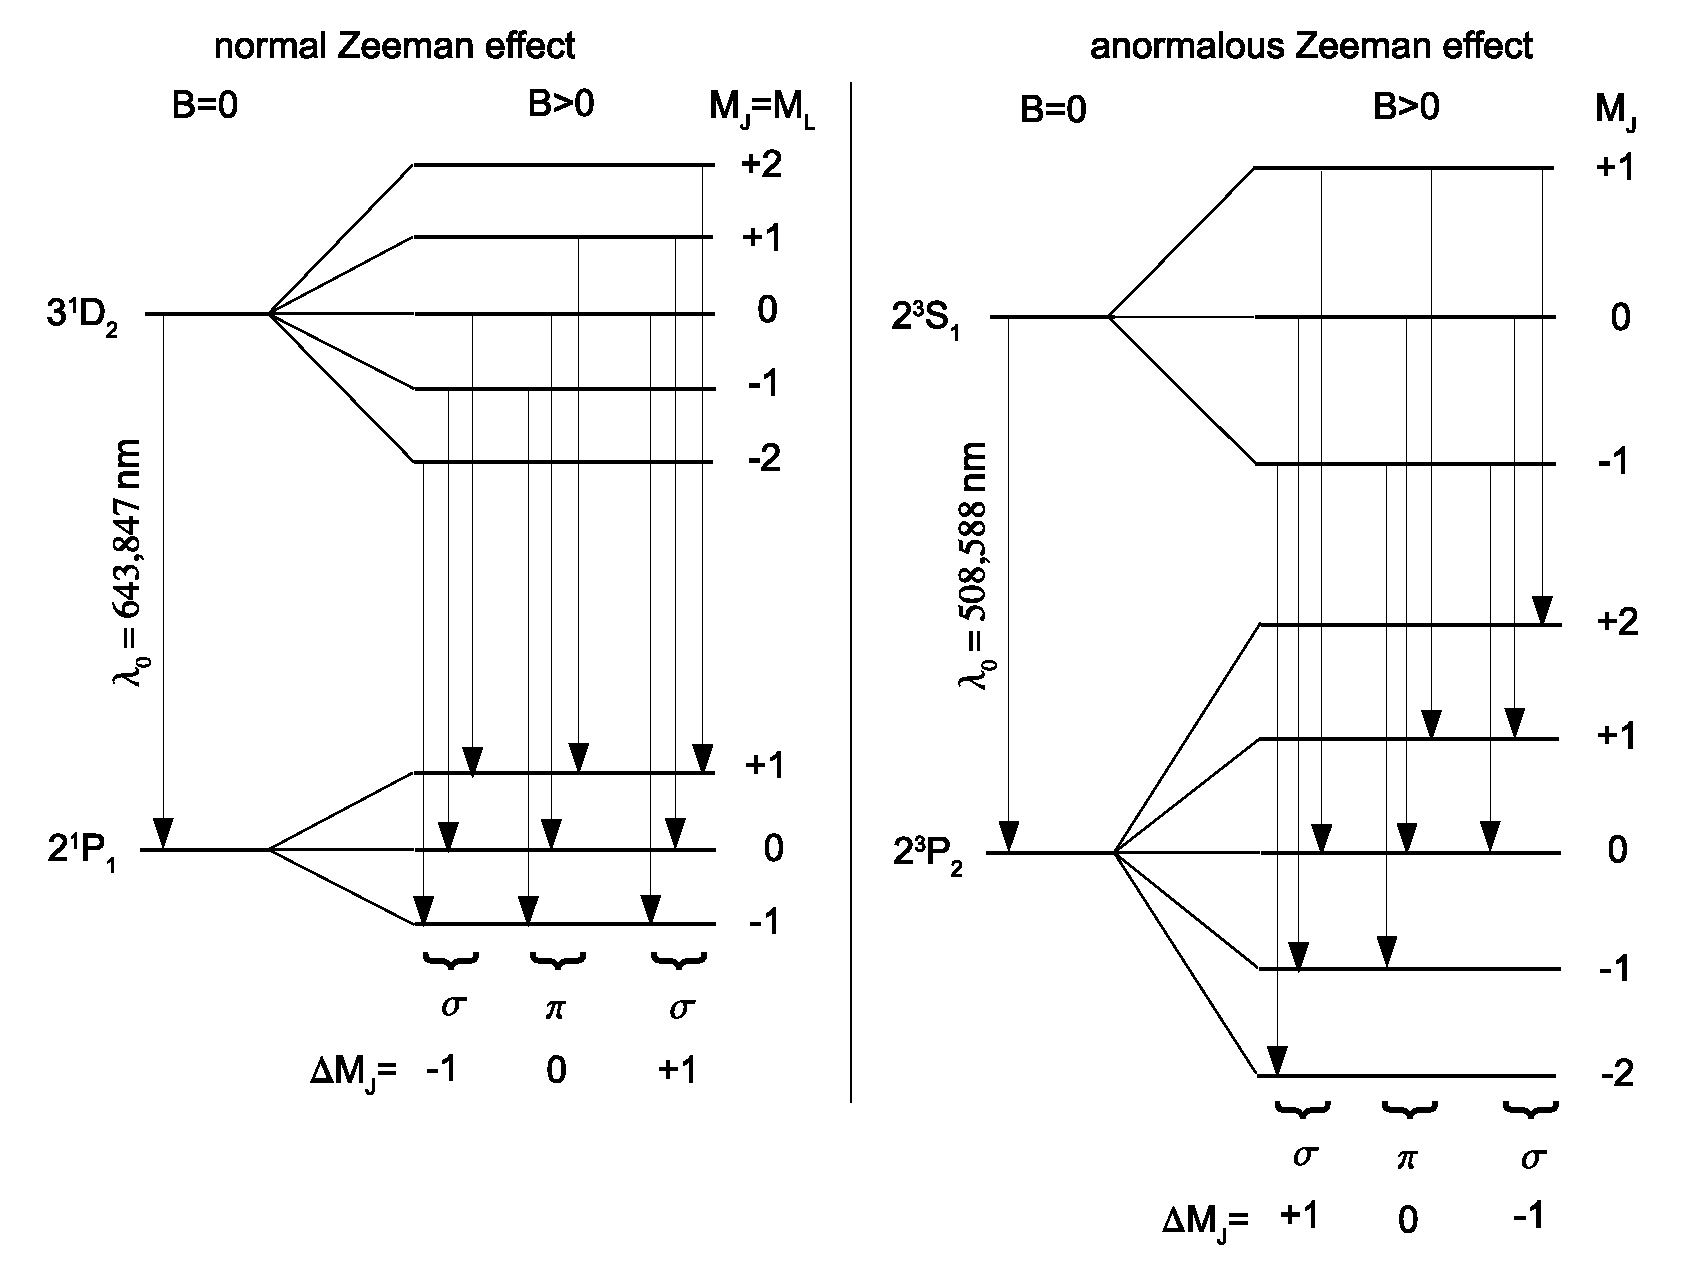
\includegraphics[width=\textwidth]{term_skizze_en}
\caption{Energy level diagram for the normal and anomalous Zeeman effect}
\label{fig:term_skizze}
\end{center}
\end{figure} 
In the state $3\,{}^1D_2$, it may $L=2$ and therefore $M_L$ can be expressed by the values $0,\pm1,\pm2$. Every one of the five state is characterized by $M_L$ and has an own individual energy in the external field $\vec{B}$ .The $2\,{}^1P_1$ states, which are triple degenerated energy levels without any field, split similarly during field presence. The distance of two neighboring levels is always $\Delta E=\mu_B B$. The selection rules for electrical dipole transitions require $\Delta M_L = 1,0,-1$. Therefore only three energetically equidistant transition energies can be observed. Fig. \ref{fig:term_skizze} shows a summary of the splitting of the both singlet states in a field and the allowed transitions. 


\subsection{Anomalous Zeeman Effect}

The anomalous Zeeman effect must be derived from a more general approach.  If an atomic system is not situated in a singlet state, the orbital angular momentum as well as the spin has to be considered. The magnetic moment of a spin is given by:

\begin{equation}
 \vec\mu_S = - g_S \frac{e}{2 m_e} \vec{S} =  - g_S \frac{\mu_B}{\hbar} \vec{S}   .
\end{equation}

$g_S \approx 2$ means the gyromagnetic factor of the spin. It is essentially a proportionality constant that relates the observed magnetic moment of an electron to the appropriate orbital angular momentum.
The norm of the total spin $\vec{S}$ in a triplet system is $|\vec{S}|=\hbar \sqrt{S(S+1)}$ for $S=1$. If the orbital angular momentum as well as the spin does not vanish concurrently in the system, the so called $L-S$-coupling has to be considered and the total angular momentum is given by:
\begin{equation}
 \vec{J}=\vec{L}+\vec{S}.
\end{equation} 

Now the magnetic moment consists of a portion for the orbital angular momentum as well as the spin but with different preliminary factors:
\begin{equation}
 \vec\mu_J=\vec \mu _L+\vec \mu_S=-\frac{\mu_B}{\hbar} (\vec{L} + 2 \vec{S}).
\end{equation} 
The total angular momentum and the magnetic moment do not remain parallel.  
By using the Land\'{e}-factor $g_J$ for the total angular momentum the potential energy in the field becomes to:

\begin{equation}
 E_{M_J}=M_J g_J \mu_B B \qquad \mathrm{mit}\qquad g_J=1+ \frac{J(J+1)+S(S+1)-L(L+1)}{2J(J+1)}  .
\end{equation}

The transitions occur in the triplet system. The two states have different $g_J$. Now the number of possible transition is nine. Fig. \ref{fig:term_skizze} summarizes the situation.

\subsection{Fabry-P\'{e}rot Interferometer}
The Fabry-P\'{e}rot interferometer generates an interference pattern by the utilization of a 3 mm thick quartz plate with coated surfaces on both sides
(90\% reflectivity, 10\% transmissivity). Fig \ref{fig:etalon_skizze} shows the optical path. 
The condition for constructive interference is 
\begin{equation}
 n\lambda = 2\mu t \cos \theta  .
\end{equation}
In this condition $n$ is an integer, $\lambda$ is the wavelength of the incident light, $\mu$ is the refractive index of the quartz plate, $t$ is the thickness of the quartz plate and $\theta$ is the angle between incident light ray and surface normal. The parallel rays $B,D,F,...$ will be focused by an optical lens with the focal length $f$. The angle satisfying the interference condition will shape a pattern of rings with the radius 
\begin{equation}  \label{eq:r_n}
 r_n = f \tan \theta_n \approx f \theta_n  .
\end{equation} 
The approximation only holds for small angles $\theta_n$.
\begin{figure}[b!]
\begin{center}
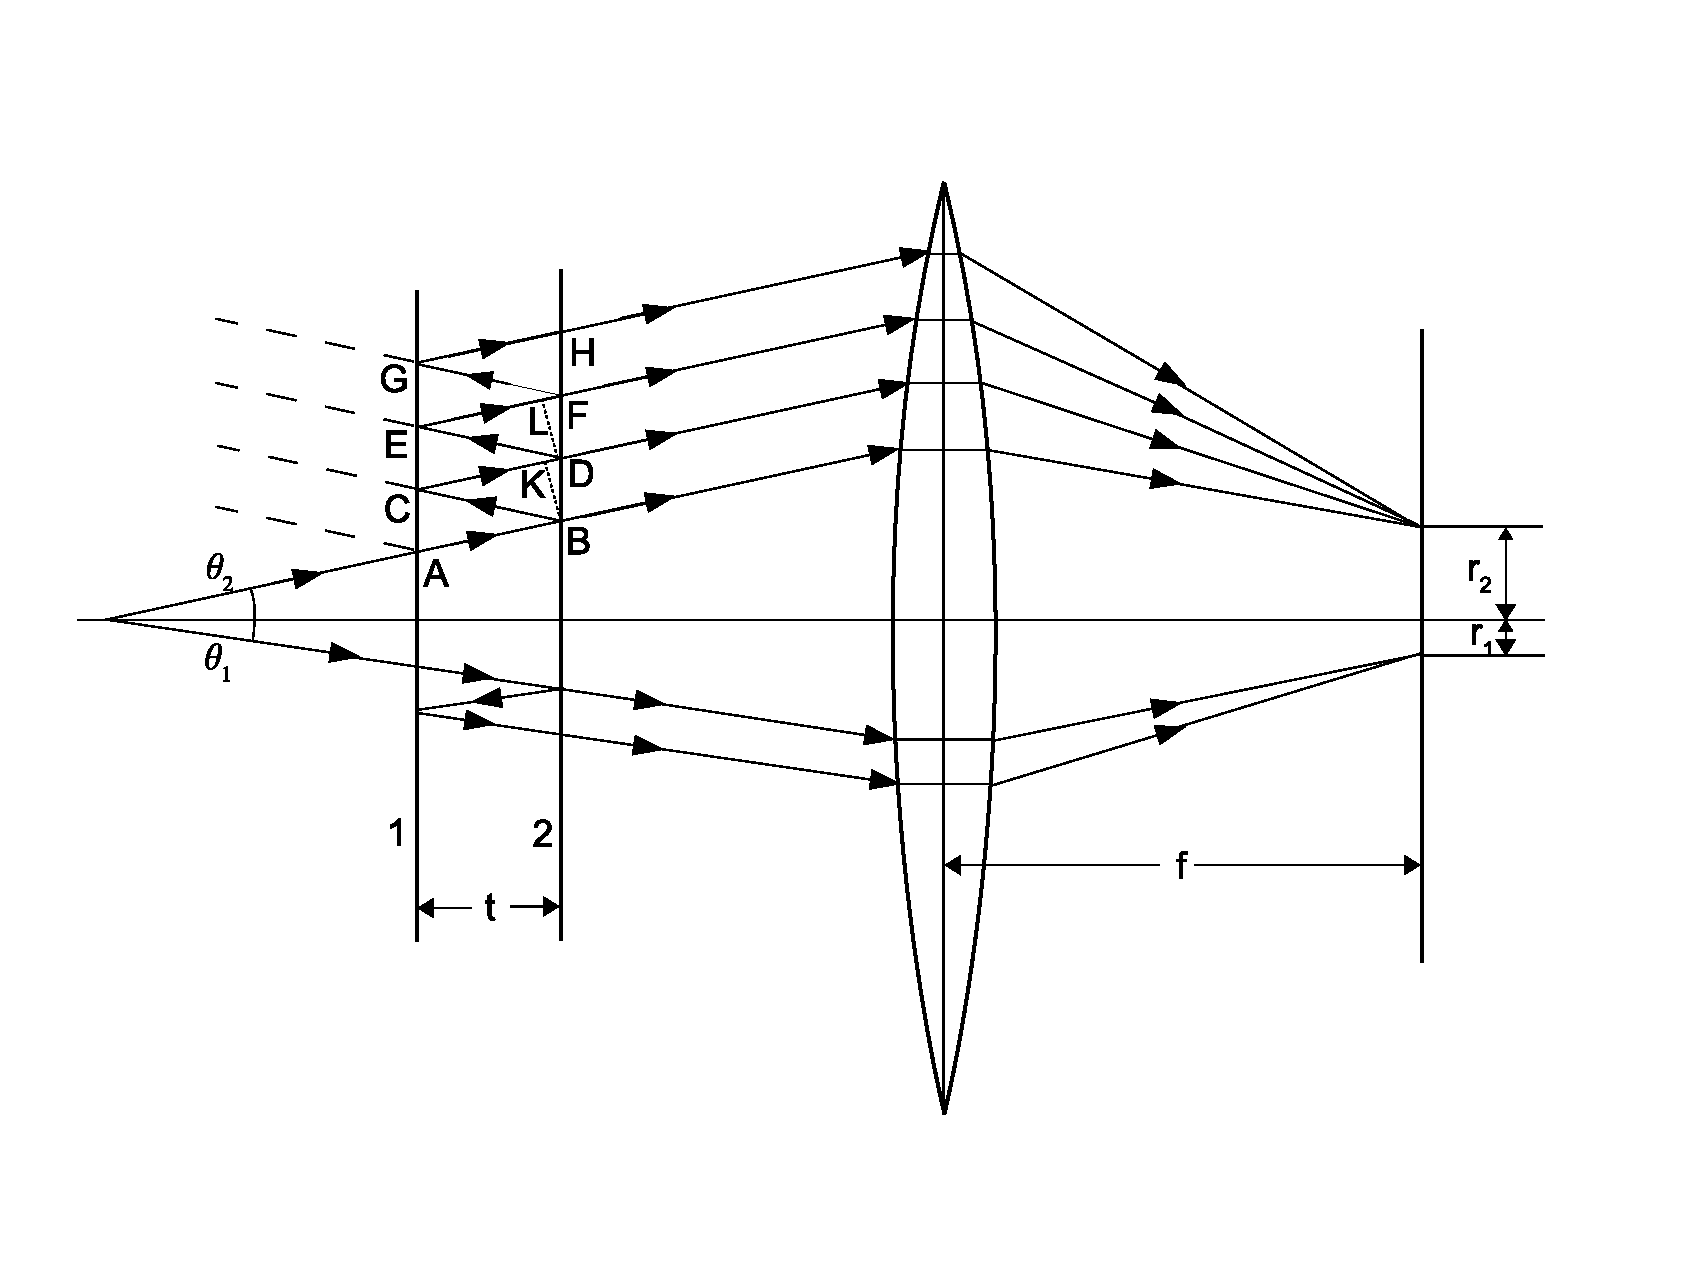
\includegraphics[width=\textwidth]{etalon_skizze}
\caption{Optical path in Fabry-P\'{e}rot interferometer with interference rings in the focal plane.}
\label{fig:etalon_skizze}
\end{center}
\end{figure}
From the interference conditions we further get: 
\begin{equation} 
n=\frac{2\mu t}{\lambda} \cos \theta_n = n_0 \cos \theta_n \approx n_0(1-\frac{\theta^2_n}{2})
\end{equation} 
with $n_0= \frac{2 \mu t}{\lambda}$. By reordering to the expression $\theta_n$, so we get
\begin{equation}  \label{eq:theta_n}
 \theta_n= \sqrt{\frac{2(n_0-n)}{n_0}}.
\end{equation}
If $\theta_n$ is the angle to a certain interference ring, so $n$ will be an integer. $n_0$ gives a condition for the center ($\theta=0$), but it is not an integer in general. By denoting the order of the first ring with $n_1$, we get
\begin{equation}
 n_1=n_0 \cos \theta_{n_1} < n_0  .
\end{equation}

Now we will define an $\epsilon$ with $0<\epsilon<1$, so that 
\begin{equation}
n_1=n_0-\epsilon  .
\end{equation}
 $n_1$ is the greatest number but still smaller than $n_0$.
If we count the rings beginning from the center, so for the $p$-th ring it is: 
\begin{equation}  \label{eq:n_p}
 n_p=(n_0-\epsilon)-(n_p-1)  .
\end{equation} 
From equations \ref{eq:r_n}, \ref{eq:theta_n} and \ref{eq:n_p} for the radius of the $p\textsuperscript{th}$ ring we get 
\begin{equation} \label{eq:rp}
  r_p=\sqrt{\frac{2f^2}{n_0}} \sqrt{(p-1)+\epsilon}  .
\end{equation} \label{eq:rp_square}
Accordingly the difference of the squared radii of two neighboring rings is constant:  
\begin{equation}  \label{eq:rp_square}
 r^2_{p+1}-r^2_p = \frac{2 f^2}{n_0}
\end{equation}
By splitting a spectral line into two closed neighboring components a and b with the wavelengths $\lambda_a$ and $\lambda_b$  for each component we get an expression for $\epsilon$:  

\begin{equation}
 \epsilon_a = \frac{2 \mu t}{\lambda_a}-n_{1,a} = \frac{\mu t k_a}{\pi} - n_{1,a} 
\end{equation} 
\begin{equation} 
  \epsilon_b = \frac{2 \mu t}{\lambda_b}-n_{1,b} = \frac{\mu t k_b}{\pi} - n_{1,b}.
\end{equation} 
 
$k_a=\frac{2\pi}{\lambda_a}$ and $k_b=\frac{2\pi}{\lambda_b}$ are the corresponding wavenumbers. $n_{1,a}$ is the interference order of the first ring for the component a and $n_{1,b}$ for the component b.
The difference of the wavenumbers can be expressed by 
 
\begin{equation} \label{eq:deltak}
 \Delta k= k_a-k_b= \pi \frac{\epsilon_a-\epsilon_b}{\mu t}  .
\end{equation}
From equation \ref{eq:rp} and \ref{eq:rp_square} we get
\begin{equation} 
 \frac{r^2_{p+1}}{r^2_{p+1}-r^2_p}-p=\epsilon  .
\end{equation} 
By applying this relation to the components a and b we get: 
\begin{equation}
 \frac{r^2_{p+1,a}}{r^2_{p+1,a}-r^2_{p,a}}-p=\epsilon_a
\end{equation}
and
\begin{equation}
 \frac{r^2_{p+1,b}}{r^2_{p+1,b}-r^2_{p,b}}-p=\epsilon_b  .
\end{equation}
By substituting equation \ref{eq:deltak} we get for the difference of the wavenumbers:
\begin{equation} \label{eq:deltak2}
 \Delta k = \frac{\pi}{\mu t}( \frac{r^2_{p+1,a}}{r^2_{p+1,a}-r^2_{p,a}}-\frac{r^2_{p+1,b}}{r^2_{p+1,b}-r^2_{p,b}}).
\end{equation}
The differences for the squared radii follow from equation \ref{eq:rp_square}:
\begin{equation}
\Delta^{p+1,p}_a=r^2_{p+1,a}-r^2_{p,a}=\frac{2f^2}{n_{0,a}}
\end{equation}
and 
\begin{equation}
\Delta^{p+1,p}_b=r^2_{p+1,b}-r^2_{p,b}=\frac{2f^2}{n_{0,b}}.
\end{equation}
For small splitting of the lines both terms can be considered equal:
\begin{equation}
 \Delta^{p+1,p}_a=\Delta^{p+1,p}_b
\end{equation}
Thus, the differences 
\begin{equation}
 \delta^p_{a,b}=r^2_{p+1,a}-r^2_{p+1,b}
\end{equation} 
should hold the same value independently from $p$. 
Regardless of the order the difference of the squared radii of different lines but same order will be simplified by the expression $\delta$.
In the same manner $\Delta$ is the difference of the squared radii of same components but neighboring order. Inserting in equation \ref{eq:deltak2} it finally results in: 
\begin{equation} \label{eq:deltak_final}
\Delta k = \frac{\pi}{\mu t} \frac{\delta}{\Delta}.
\end{equation}
Now this equation is independent from the dimension of the different radii!  


\section{Experiment}
\subsection{Calibration of the Magnet and Adjustment of the Spectrometer }
In this experiment the Zeeman effect will be demonstrated by using the light of a cadmium lamp in a magnetic field of a permanent magnet. 
The distance between the pole pieces of the magnet can be changed and thereby the amount of the magnetic flux density $B$. For operating with defined field values later the magnetic flux density has to be calibrated by using a Hall effect sensor at first. By employing a red optical filter a narrow range around the $\lambda_n=643,847 \;\mathrm{nm}$ line will be selected from all obtainable atomic transitions. This atomic transition can be resolved by using a Fabry-P\'{e}rot etalon and regarding to the magnetic field the transversal and longitudinal splitting can be observed. In the setup for longitudinal observations the optical axis is parallel to the magnetic field and the drilling in the pole piece acts as a light source. In the experiments for transversal observations instead of the drilling an additional iris aperture is used for establishing a light source. 
The almost parallel light path required for interference is generated with the lens $L_1$ and along with the fixed lens $L_{FPE}$ with a focal length of $f=100 \;\mathrm{mm}$. The lenses $L_2$ and $L_3$ act as a telescope, whose image is recorded by CCD camera and evaluated by PC. Fig. \ref{fig:aufbau_bank_skizze} shows the arrangement of the various optical components and the corresponding approximated positions for longitudinal setup.  
The geometry of the setup has to be varied until the camera gets a sharp image. 
\begin{figure}[!h] 
\begin{center}
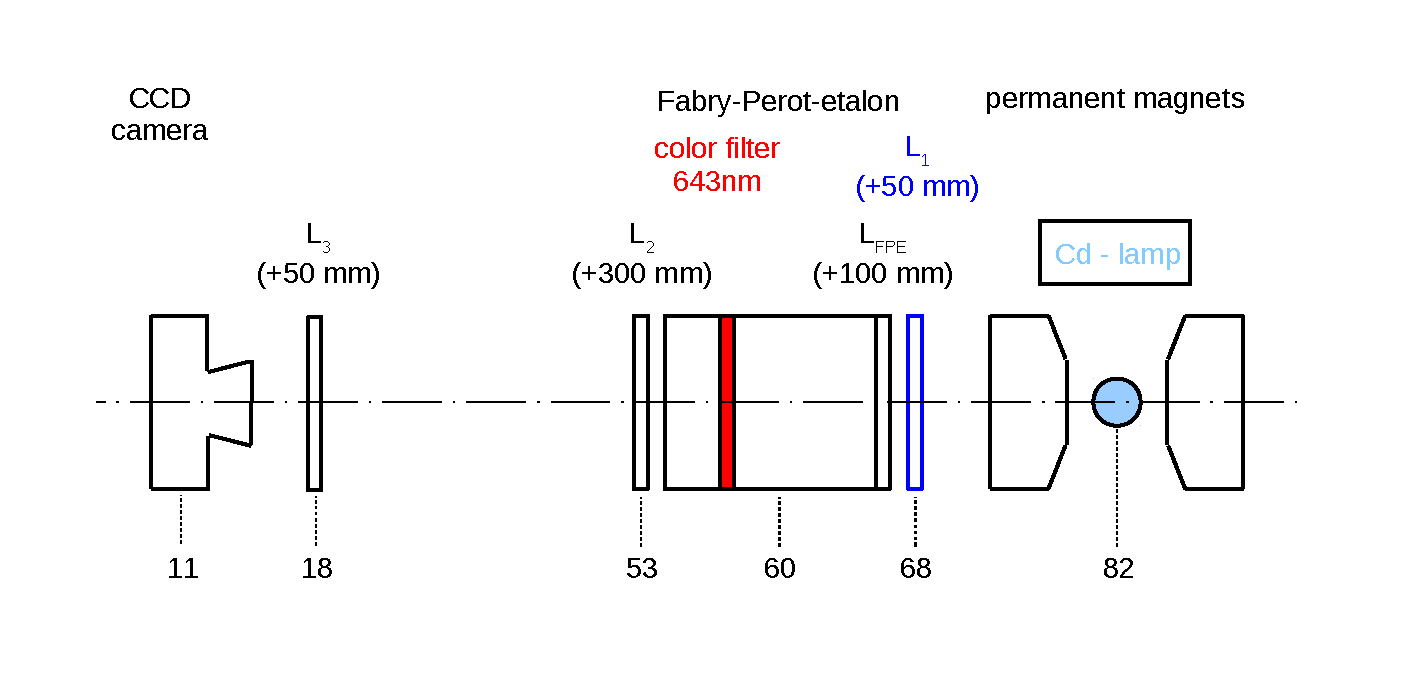
\includegraphics[width=\textwidth]{aufbau_bank_right_engl}
\caption{Longitudinal setup with optical components and corresponding approximated positions (in cm) for observation of the red $\lambda_n=643,847 \;\mathrm{nm}$ line}
\label{fig:aufbau_bank_skizze}
\end{center}
\end{figure} 

\subsection{Normal Zeeman Effect: Polarization}
At electrical dipole transitions the selection rule for the total angular momentum component is $\Delta M_J= 0, \pm 1$. Transitions according to $\Delta M_J=0$ are called $\pi$-lines and suchlike according to $\Delta M_J= \pm 1$ are called $\sigma$-lines. 
By inserting a polarizing filter between $L_2$ and $L_3$ different polarization directions can be selected. Modify the setup to transversal geometry and put in the iris aperture at the former position the drilling in pole piece. Without polarizing filter three optical transitions can be observed in the case of normal Zeeman effect. Meanwhile with a vertical polarizing filter only $\sigma$-lines and with a horizontal polarizing filter only $\pi$-lines can be observed. Write down your own observation for each case. 
By changing to the longitudinal setup two lines are visible independent from polarizer angle. The $\pi$-transitions are unobservable in the longitudinal setup. A $\lambda/4$ plate transforms circularly polarized light to a linear polarization. After light passage the direction of the polarization is rotated by $\pi / 4$ regarding to the optical axis of the plate. Afterwards to demonstrate the initial circularly polarization the polarizer can be rotated regarding to the optical axis of the $\lambda/4$ plate. Put in the $\lambda/4$ plate between $L_2$ and the polarizer and write down your observations for various polarizer angles. Fig. \ref{fig:polarisations_skizze} summarizes the polarization effect of the optical transitions in a magnetic field.

\begin{figure}[!h] 
\begin{center}
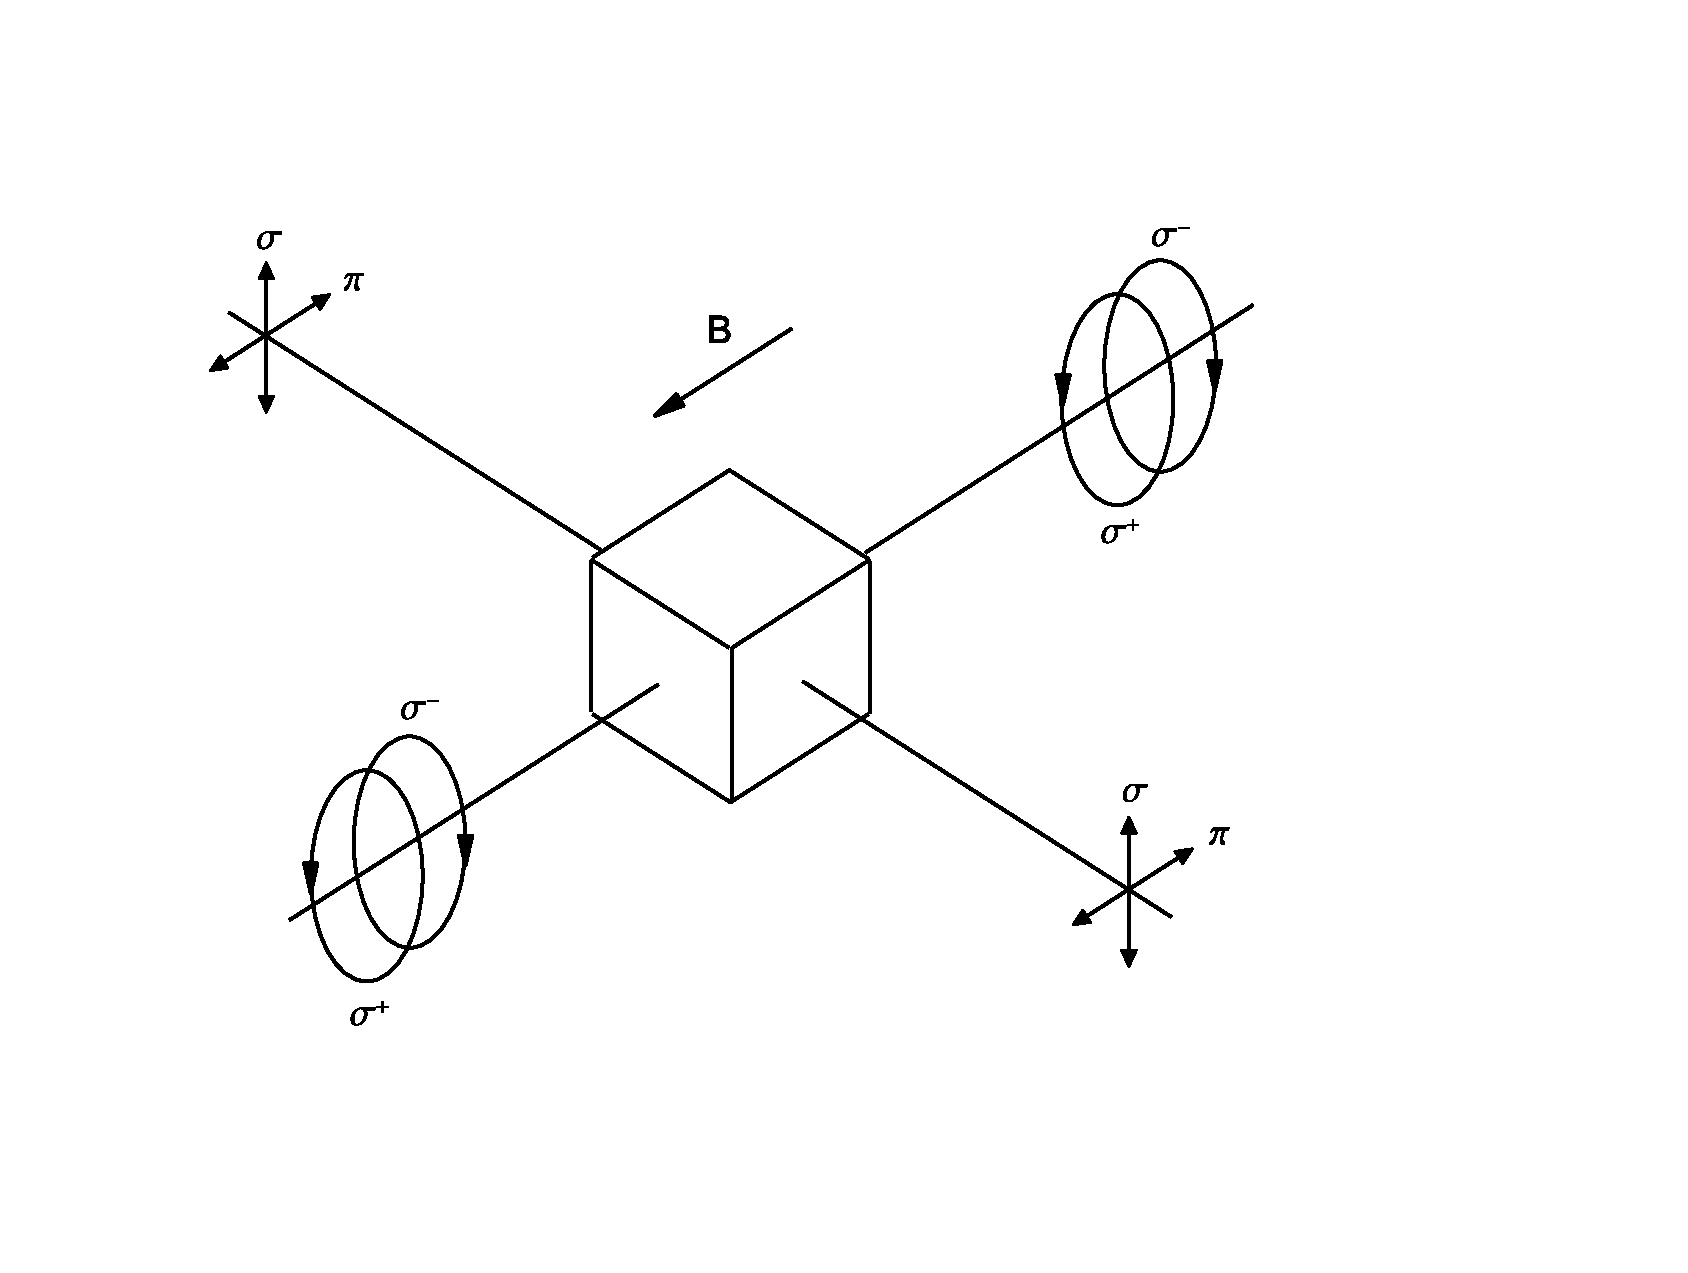
\includegraphics[width=\textwidth]{polarisations_skizze}
\caption{Polarization in longitudinal and transversal direction of observation}
\label{fig:polarisations_skizze}
\end{center}
\end{figure} 


\subsection{Normal Zeeman Effect: Determination of the Bohr Magneton}
Considering the derived equations from the theoretical chapter the line splitting in the magnetic field can be determined quantitatively depending on the magnetic flux density. For that use the transversal setup and determine the enclosed ring area at the first three interference orders and at five different field intensities between $150 \, \mathrm{mT}$ and $450 \, \mathrm{mT}$.
The area is proportional to the squared radius, the factor $4 \pi$ can be reduced in eq. \ref{eq:deltak_final}.
Plot the relation $\Delta E = h \Delta f$ in dependence of $B$ by using the average of the areas ($c=2,99 \;10^8 \frac{\mathrm{m}}{\mathrm{s}}$, $h=6,626 \;10^{-34}\frac{\mathrm{J}}{\mathrm{s}}$). 
Determine $\mu_B$ for each field intensity and compare your result the literature value $\mu_B = 9,273 \;10^{-24} \frac{\mathrm{J}}{\mathrm{T}}$. The refractive index of the quartz plate of the etalon is $\mu_{\mathrm{644 nm}} = 1,4560$ ( $\mu_{509 \mathrm{nm}}=1,4519$). The thickness of the plate is $t=3 \mathrm{mm}$.


\subsection{Anomalous Zeeman Effect }
In the magnetic field complicated interference pattern can be observed for transitions of the green $\lambda_n=508,588 \;\mathrm{nm}$ line. Remove the red optical filter and install the green filter at lens $L_2$. Repeat the experiments for the polarization with longitudinal and transversal setup. Compare your results with the properties of the participating $2^3S_1$ and $2^3P_2$ states and with your results regarding the normal Zeeman effect.


\frage{How is the functionality of a $\lambda / 4$ plate, of a polarizer filter and of an interference filter?}
\frage{How is the generation of the interferences at a Fabry-P\'{e}rot etalon?}
\frage{Familiarize yourself with the energy level diagrams to the Zeeman effect. What are the differences between the line splitting at the normal and at the anomalous Zeeman effect?}


\end{document}


